\documentclass{jsarticle}
\usepackage[dvipdfmx]{graphicx}
\title{真空プロセスによる薄膜作製}

\author{03-190697 高松周平}
\date{\today}
\begin{document}
\maketitle
\section{概要}
\subsection{実験の目的}
真空を使った薄膜作製を行うことで真空の理解を深める。また、作製した薄膜の特性なども学ぶ。\\
\subsection{原理}
\subsubsection{真空ポンプ}
\begin{itemize}
\item \textbf{油回転ポンプ(ロータリーポンプ, RP)}\\
\ 低真空用のポンプ。偏心したしたローターを回転させ吸入気体を圧縮して外部に排出することで真空をつくる。到達圧力は最高$10^{-1}$Pa程度。
\item \textbf{油拡散ポンプ(ディフュージョンポンプ, DP)}\\
\ 高真空用のポンプ。気化させた油を超音速ジェットとして下向きに噴出させることで、吸入した気体分子を巻き込み排気口まで輸送することによって真空をつくる。油は側面で冷却され装置底部に戻る。原理上$10$Pa以上では動作しないので前述の油回転ポンプを用いてから使う。到達圧力は$10^{-4}$〜$10^{-5}$Pa程度である。また動作中は必ず冷却しなければならない
\end{itemize}
\subsubsection{真空計}
\begin{itemize}
\item \textbf{低真空用:ブルドン管(差圧計)}
\item \textbf{低真空用:ピラニ真空計}
\item \textbf{中真空用:隔膜真空計}
\item \textbf{高真空用:電離真空計}
\end{itemize}
\subsubsection{真空蒸着法}
\ 真空蒸着法は薄膜作製法の中で最も簡便な方法の一つ。薄膜として得たい物質を真空中の低部で加熱し蒸発させ、その蒸気を上部に設置した基盤の表面に吸着させ凝縮させることによってその物質の薄膜を得ることができる。また、いくつかの理由から、これらを行うのは真空環境で行われる。まず、高温の蒸着源がベルジャー内の気体分子と反応することを防ぐため、次に気体分子と衝突することにより蒸発物質の基盤表面への到達が妨げられたり、気相中で凝縮する原因になるのでそれを防ぐため、最後に気体分子の薄膜への混入を防ぐためである。当然真空を維持し蒸発した物質が四方へ飛ぶのを防ぐために、ベルジャーはガラスでできた容器で覆われている。\\
\ 気相中の気体分子の衝突から次の衝突までの平均移動距離を平均自由工程$\lambda$というが、この値は分子半径、温度、圧力に依存し、分子半径を$0.2$nmとすると常温($300$K)では
$$
\lambda=\frac{6.6\times 10^{-3}}{P[Pa]}
$$
となるここで、蒸着源と基盤の距離を$L$とすると、$\lambda / L$はクヌーセン数($Kn$)とよばれ、基盤到着までの気体分子の衝突の程度すなわち、気体の流れを評価する指標となる。\\
\ また、薄膜として得たい物質の平衝蒸気圧も重要な因子となる。蒸着速度は蒸発する分子数に比例する。つまり、蒸気圧の低い物質は一定の蒸着速度を得るために、高温を保たねばならず、真空蒸着法が難しい。
\subsubsection{薄膜作製の初期過程}
\ 薄膜形成には規則性が生じるがそれは、初期過程に起因する。主に、三種類にわけられる。三次元核生成、単層成長、単層上核生成とあり、今回のAuも含め多くの物質は最初の三次元核生成に分類される。
\subsection{手順}
\subsubsection{真空蒸着によるAu薄膜の作製}
\begin{itemize}
\item ベルジャー内は初期状態で真空なのでまず大気圧にする。
\item ベルジャー内に蒸発物質と基盤を設置しベルジャー内を各種ポンプを用いて真空にする。
\item 蒸着源を加熱し蒸着を開始する。
\item ゆっくりと冷却し、ベルジャー内を大気圧に戻し、基盤を取り出す。
\item 最後にベルジャー内を粗排気しておく。
\end{itemize}
\subsubsection{四深針法にAu薄膜の抵抗率測定}
\begin{itemize}
\item 標準試料としてAu板(正方形、膜厚0.2mm)の抵抗率を評価する。
\item 次に、得られた試料の抵抗率を測定する。
\end{itemize}
\subsubsection{原子間力顕微鏡(AFM)によるAu薄膜の膜圧測定}
\begin{itemize}
\item 得られた試料の中央部をケガキ溝を作る。
\item この溝をAFMで測定し断面ラインプロファイルを得る。
\item これを用いて高低差を求め、試料の膜厚を計算する。
\end{itemize}
\subsubsection{気体の熱伝導の圧力依存性測定(真空断熱)}
\begin{itemize}
\item 油拡散ポンプの排気速度を測定する。
\item ベルジャー圧力を$10^{-2}$Pa〜$10^{4}$Paまで変化させそれぞれ五分間保持した後にヒーターと500$\mu$m離れて対向する銅プレートの温度を記録する。
\item ヒーターと銅プレートの温度差から気体の熱伝導の圧力依存性を把握する。
\end{itemize}
\section{実験結果(薄膜)}
\subsection{AFM断面図}
\begin{figure}[htbp]
 \begin{minipage}{0.5\hsize}
  \begin{center}
   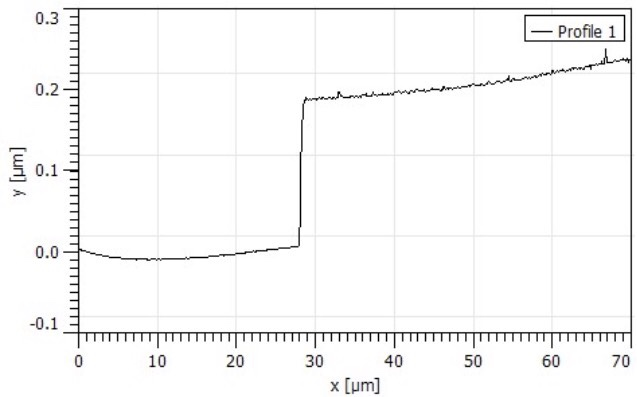
\includegraphics[width=70mm,height=35mm]{pictures/01.jpg}
  \end{center}
 % \caption{No.1}
  \label{fig:one}
 \end{minipage}
 \begin{minipage}{0.5\hsize}
  \begin{center}
   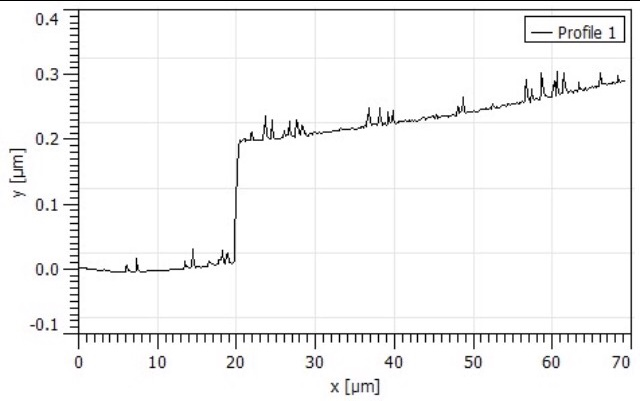
\includegraphics[width=70mm,height=35mm]{pictures/02.jpg}
  \end{center}
%  \caption{No.2}
  \label{fig:two}
 \end{minipage}
\end{figure}
\begin{figure}[htbp]
 \begin{minipage}{0.5\hsize}
  \begin{center}
   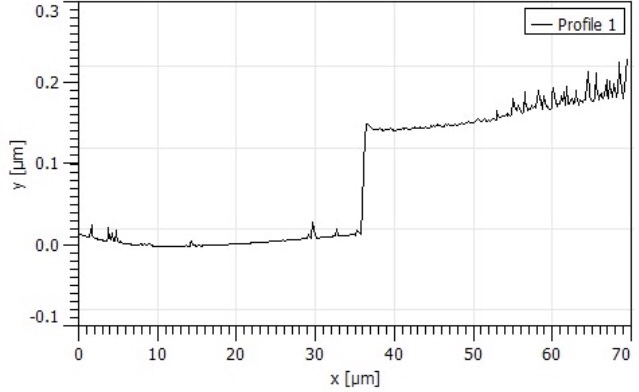
\includegraphics[width=70mm,height=35mm]{pictures/03.jpg}
  \end{center}
%  \caption{No.3}
  \label{fig:one}
 \end{minipage}
 \begin{minipage}{0.5\hsize}
  \begin{center}
   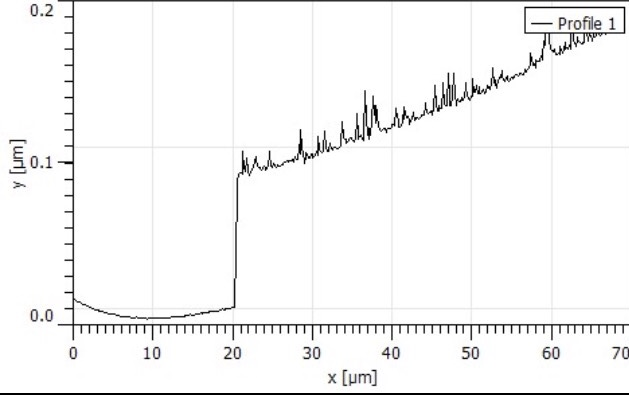
\includegraphics[width=70mm,height=35mm]{pictures/04.jpg}
  \end{center}
%  \caption{No.4}
  \label{fig:two}
 \end{minipage}
\end{figure}
\begin{figure}[htbp]
 \begin{minipage}{0.5\hsize}
  \begin{center}
   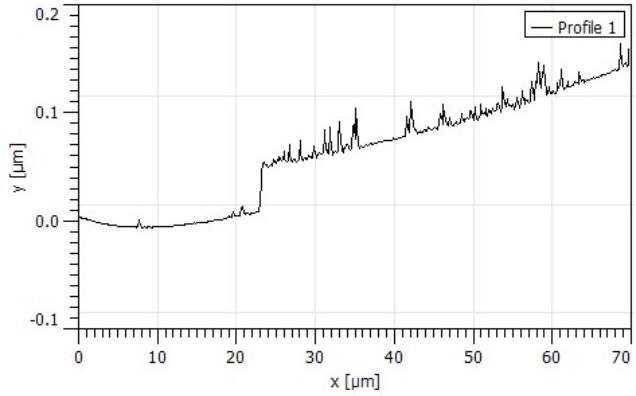
\includegraphics[width=70mm,height=35mm]{pictures/05.jpg}
  \end{center}
%  \caption{No.5}
  \label{fig:one}
 \end{minipage}
 \begin{minipage}{0.5\hsize}
  \begin{center}
   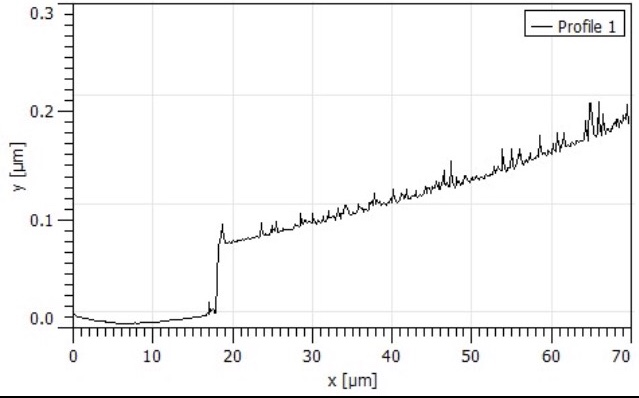
\includegraphics[width=70mm,height=35mm]{pictures/06.jpg}
  \end{center}
%  \caption{No.6}
  \label{fig:two}
 \end{minipage}
\end{figure}
\begin{figure}[htbp]
 \begin{center}
  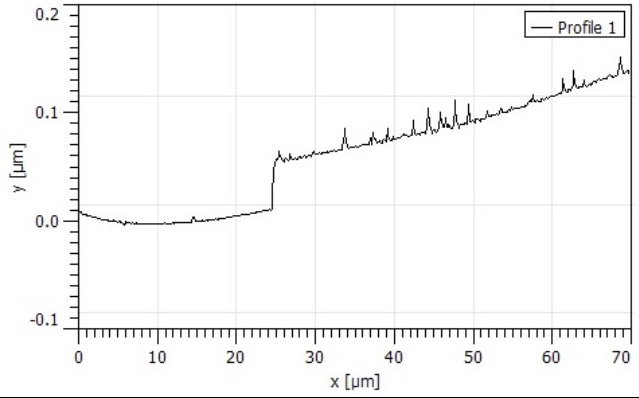
\includegraphics[width=70mm,height=35mm]{pictures/07.jpg}
 \end{center}
% \caption{No.7}
 \label{fig:one}
\end{figure}
\ 
\subsection{蒸着源からの距離と膜厚の関係}
\ 
\begin{figure}[htbp]
 \begin{minipage}{0.5\hsize}
  \begin{center}
   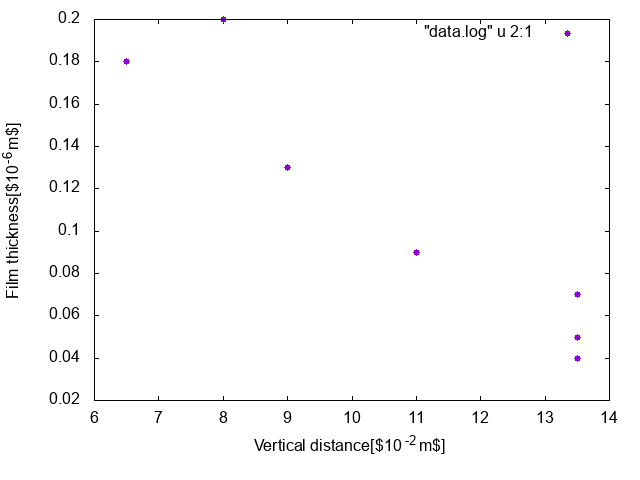
\includegraphics[width=70mm,height=35mm]{pictures/graph01.png}
  \end{center}
%  \caption{No.5}
  \label{fig:one}
 \end{minipage}
 \begin{minipage}{0.5\hsize}
  \begin{center}
   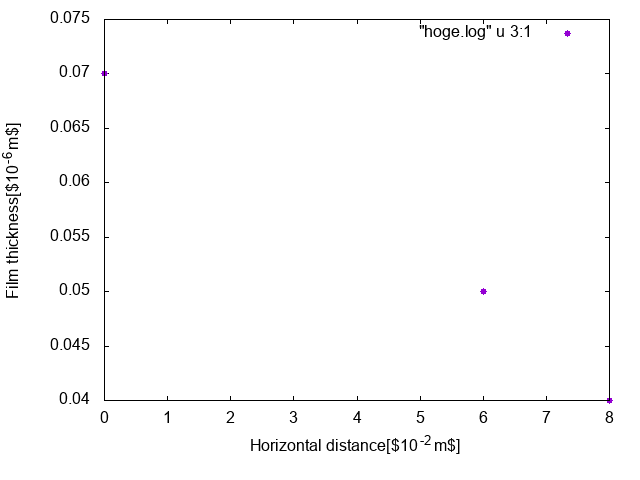
\includegraphics[width=70mm,height=35mm]{pictures/graph02.png}
  \end{center}
%  \caption{No.6}
  \label{fig:two}
 \end{minipage}
\end{figure}
\subsection{抵抗率の計算}
$シート抵抗Rs=Cs(\frac{V}{I})$\ (Cs:実験サンプル4.12,標準サンプル4.5324)よりRsを求める。そして、それをもとに$抵抗率\rho=Rs\cdot d(膜厚)$を求める。\\
またこのとき最小二乗法を用いる。$y=ax, a=\frac{n\sum{xy}-\sum{x}\sum{y}}{n\sum{x^2}-(\sum{x})^2}$を用いる。\\
Auの抵抗率の文献率は$2.35\times10^{-6}[\Omega\cdot cm]$\\
よってこの式に当てはめていくと、以下の表のようになる。\\
\begin{table}[h]
\caption{各試料の抵抗率}
 \label{table:SpeedOfLight}
 \centering
  \begin{tabular}{clll}
   \hline
   番号 & Rs[$\Omega$] & d[$\mu\cdot m$] & $\rho[\mu\cdot\Omega\cdot cm]$ \\
   \hline \hline
    0 & 0.01189 & 200 & 2.38 \\
    1 & 0.234 & 0.179 & 4.19\\
    2 & 0.230 & 0.20 & 4.60\\
    3 & 0.334 & 0.13 & 4.35\\
    4 & 0.543 & 0.09 & 4.88\\
    5 & 1.672 & 0.038 & 6.356\\
    6 & 0.808 & 0.075 & 6.06\\
    7 & 1.214 & 0.046 & 5.583\\
   \hline
  \end{tabular}
\end{table}
\\
またすべての試料について電流と電圧の関係をプロットしたのが次の図である。\\
上の図より大体オームの法則に従ってると言える。\\
また、シート抵抗と抵抗率の関係をグラフにしたのが次の図である。
\\
\begin{figure}[htbp]
 \begin{minipage}{0.5\hsize}
  \begin{center}
   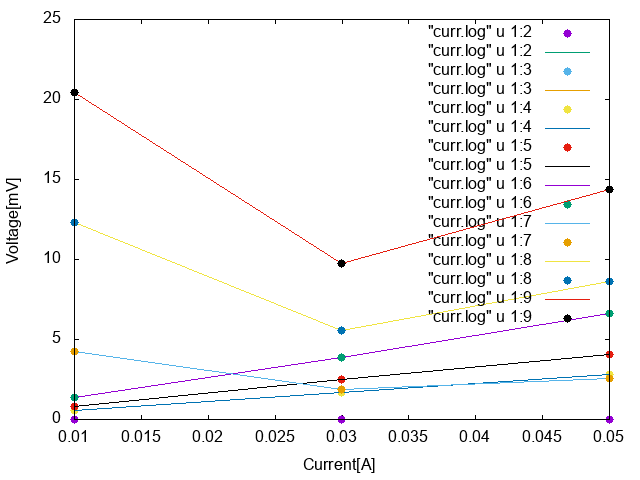
\includegraphics[width=70mm,height=35mm]{pictures/curr-volt.png}
  \end{center}
%  \caption{No.5}
  \label{fig:one}
 \end{minipage}
 \begin{minipage}{0.5\hsize}
  \begin{center}
   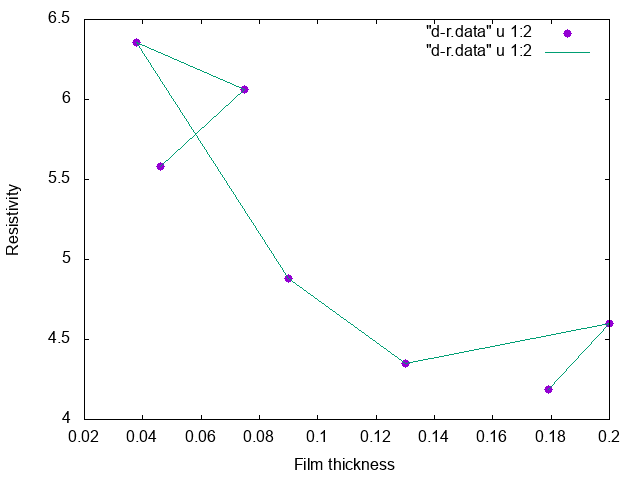
\includegraphics[width=70mm,height=35mm]{pictures/d-r.png}
  \end{center}
%  \caption{No.6}
  \label{fig:two}
 \end{minipage}
\end{figure}
\\
\section{結果考察(薄膜)}
\subsection{}
グラフより、水平方向、鉛直方向ともに理論通り蒸着源から離れるほどその距離に比例して膜厚は薄くなっている。
\subsection{}
文献値が$2.35\times10^{-6}[\Omega\times cm]$なのでそれに比べ非常に大きい値になっている。膜が薄いほど大きい値になっている。
\subsection{}
電解エネルギーが試料の外に出られないので膜厚が薄いほど、抵抗値が大きく計測されたと思われる。
\section{実験結果(熱伝導)}
各圧力における銅プレートの温度差のグラフが以下である。\\
\begin{figure}[htbp]
 \begin{center}
  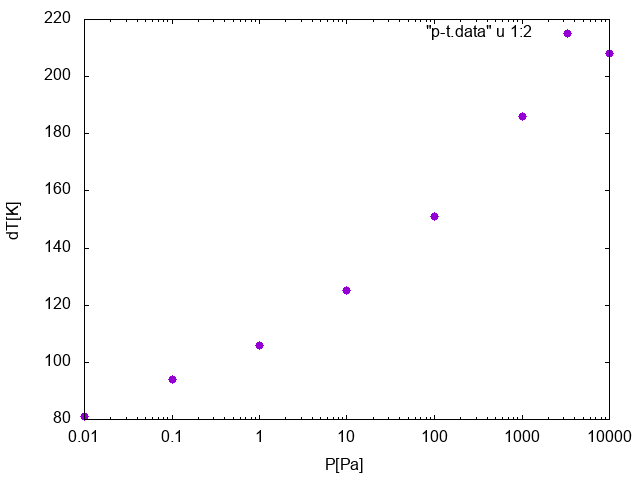
\includegraphics[width=70mm,height=35mm]{pictures/p-t.png}
 \end{center}
% \caption{No.7}
 \label{fig:one}
\end{figure}
\section{結果考察(熱伝導)}
\subsection{}
以下の表をもとに考えると、P $>10^3$のとき粘性流、P$<1.0$のとき分子流、間のとき遷移領域である。
\begin{table}[h]
\caption{各圧力におけるクヌーセン数}
 \label{table:SpeedOfLight}
 \centering
  \begin{tabular}{clll}
   \hline
   圧力[Pa] & Kn \\
   \hline \hline
    $10^{-2}$ & $1.32\times10^{3}$ \\
    $10^{-1}$ & $1.32\times10^{2}$ \\
    $1.0$ & $1.32\times10^{1}$ \\
    $10^{1}$ & $1.32$ \\
    $10^{2}$ & $1.32\times10^{-1}$ \\
    $10^{3}$ & $1.32\times10^{-2}$ \\
    $10^{4}$ & $1.32\times10^{-3}$ \\
   \hline
  \end{tabular}
\end{table}
\subsection{}
熱伝導の圧力依存性は大まかにKnに正しいと思われる。グラフより低圧力下では線形領域であり、1気圧あたりから線形領域を抜けて、$10^{4}$気圧あたりで頭うっているのがわかる。
\section{問題}
\subsection{}
長時間真空を維持しようとすると容器内が油の蒸気で満たされてしまうから。\\
\subsection{}
上と同様で長時間真空を維持しようとすると容器内が油の蒸気で満たされてしまうから。\\
\subsection{}
$$
\overline{v}=\sqrt{\frac{3RT}{M\times10^{-3}}}と表せる。\\
$$
$$
空気の分子量は約28.8なのでM=28.8,T=300R=8.31429を代入すると、\overline{v}=161.1
$$
$$
六方向について考えるので、J=6.0\times10^{23}\times161.1/6 = 1.611\times10^{25}
$$
$$
A=0.04\times0.04\times\pi=0.005
$$
$$
S=1.611\times10^{25}\times0.005=8.055\times10^{22}
$$
以降わかりませんでした
\subsection{}
\subsection{}
\subsection{}
\begin{figure}[htbp]
 \begin{center}
  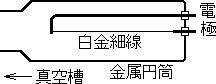
\includegraphics[width=70mm,height=35mm]{pictures/PIRANI.png}
 \end{center}
% \caption{No.7}
 \label{fig:one}
\end{figure}
上の図のような構造をしており、電極を通じて細線に電流を流すと熱Qが生じる。定常状態では、
$$
Q=Q_g + Q_r + Q_s \ \   
Q_g:自由分子の熱伝導による熱,Q_r:輻射の放射熱,Q_s:電極への固体熱伝導による熱\\
$$
が成り立つ。このとき細線と金属円筒ないの温度が一定としたとき$Q_rとQ_s$は定数になる。また$Q_g$は$Q_g=Ap$と定数Aによって気圧に比例する。そして、$Q=IR^2$とQは制御できるのでPを計算することができる。\\
しかし$Kn<0.1$の粘性流領域では熱伝導が気圧に依存しなくなるのでこの計測は行えない。
\subsection{}
上限:$10^1$Paオーダー、下限:$10^{-1}$Paオーダー\\
ピラニ真空計は気体の平均自由工程が細線の直径よりも十分大きくなくてはならないので上限が存在する。\\
固体熱伝導と輻射によって0.1オーダー以上の精度はでない\\
\subsection{}
まず、窒素ガスがばらまかれるのを防ぐためにタンクの栓をしめる。そして油拡散ポンプの冷却が止まってしまうので油拡散ポンプを停止させる。
\section{参考文献}
\begin{thebibliography}{99}
\bibitem{} 教科書
\bibitem{} 気体分子の入射頻度 http://www.nucleng.kyoto-u.ac.jp/people/ikuji/edu/vac/app-A/gas-flux.html
\bibitem{} 真空ポンプの原理と排気速度 http://www.nucleng.kyoto-u.ac.jp/people/ikuji/edu/vac/app-A/pspeed.html
\bibitem{} ピラニ真空計http://www.nucleng.kyoto-u.ac.jp/people/ikuji/edu/vac/chap3/pirani.html
\end{thebibliography} 
\end{document}
